\documentclass[11pt, letterpaper]{article}
\usepackage{graphicx}
\usepackage[a4paper, margin=4em, footskip=2em]{geometry}
\usepackage{parskip}

\title{
    Implementační dokumentace k 2. úloze do IPP 2023/2024 \\
    Jméno a příjmení: Michal Cenek \\
    Login: xcenek04
}
\date{}

\begin{document}

\maketitle

\section{Návrh}

Pro každou instrukci je definovaná třída, která dědí z abstraktní třídy \texttt{Instruction} a implementuje metodu \texttt{execute}. Interpret má seznam instrukcí a pro každou volá její metodu \texttt{execute}, které předá objekty typu \texttt{InterpreterContext} a \texttt{IO}. \texttt{InterpreterContext} obsahuje informace o stavu interpretu včetně datových rámců, datového zásobníku a zásobníku volání. \texttt{IO} umožňuje číst ze standardního vstupu a vypisovat na standardní a chybový výstup.

Hodnoty jsou reprezentovány třídou \texttt{Value}. Ta uchovává informaci o tom, jestli je hodnota inicializovaná a hodnotu, která může nabývat více typů. Dále má metody pro bezpečnou práci s těmito typově dynamickými hodnotami.

\section{Implementace}

\subsection{\texttt{Instruction}}

Instrukce má \texttt{opcode}, ke které zle přistupovat pomocí metody \texttt{getOpcode}. Podtřídy mají argumenty typu \texttt{Argument}, která uchovávají typ argumentu a jeho text, přesně ve tvaru, ve kterém byl přečten ze vstupního XML souboru.

\subsection{\texttt{Argument}}

Objekty tohoto typu uchovávaní enum \texttt{IPPType} reprezentující typ argumentu a text argumentu. Text je uložen v původním tvaru, ve kterém byl přečten ze vstupního XML souboru.

\subsection{\texttt{InstructionFactory}}

Třída \texttt{InstructionFactory} implementuje metodu \texttt{create}, která vytvoří instanci instrukce podle zadaného \texttt{opcode} a pole argumentů.

\subsection{\texttt{InterpreterContext}}

Třída \texttt{InterpreterContext} uchovává informace o stavu interpretu. Obsahuje datové rámce, datový zásobník, zásobník volání, informaci o tom, jestli má vykonávání instrukcí pokračovat a kód chyby, který se má vrátit. Obsahuje metody pro práci s těmito daty.

\subsection{\texttt{IO}}

Třída \texttt{IO} zapouzdřuje \texttt{InputReader} a \texttt{OutputWriter} z \textit{ipp-core}.

\subsection{\texttt{Frame}}

\texttt{Frame} reprezentuje datový rámec. Informace o symbolech uchovává v asociativním poli, které mapuje řetězce na \texttt{Value}. Metody umožňují definici proměnné, přiřazení a získání její hodnoty.

\subsection{\texttt{Value}}

Objekty typu \texttt{Value} uchovávají logickou hodnotu, která uruje, zda je hodnota inicializovaná, a hodnotu, která může být typu \texttt{int}, \texttt{bool}, \texttt{string} nebo \texttt{null} (\texttt{null} reprezentuje \texttt{nil} jazyka \texttt{IPPcode24}). Implementuje metody pro aritmetické, logické a řetězcové operace, pro kontrolu dynamického typu a pro nastavení a získání hodnoty.

\subsection{\texttt{Interpreter}}

Třída \texttt{Interpreter} implementuje metodu \texttt{execute}. Ta nejdřív zavolá soukromou funkci \texttt{parseXML}, která načte XML soubor a vytvoří seznam instrukcí. Poté vytvoří instanci \texttt{InterpreterContext} a \texttt{IO} a pro každou instrukci zavolá její metodu \texttt{execute}. Proměnná \texttt{programCounter} určuje index instrukce, která se má vykonat. Po vykonání každé instrukce se \texttt{programCounter} inkrementuje a skokové instrukce mohou tuto hodnotu změnit.

\subsection{Výjimky}

Pro každý typ chyby je definována výjimka dědící z \texttt{IPPException}.

\vspace{6em}

\begin{figure}[h]
  \centering
  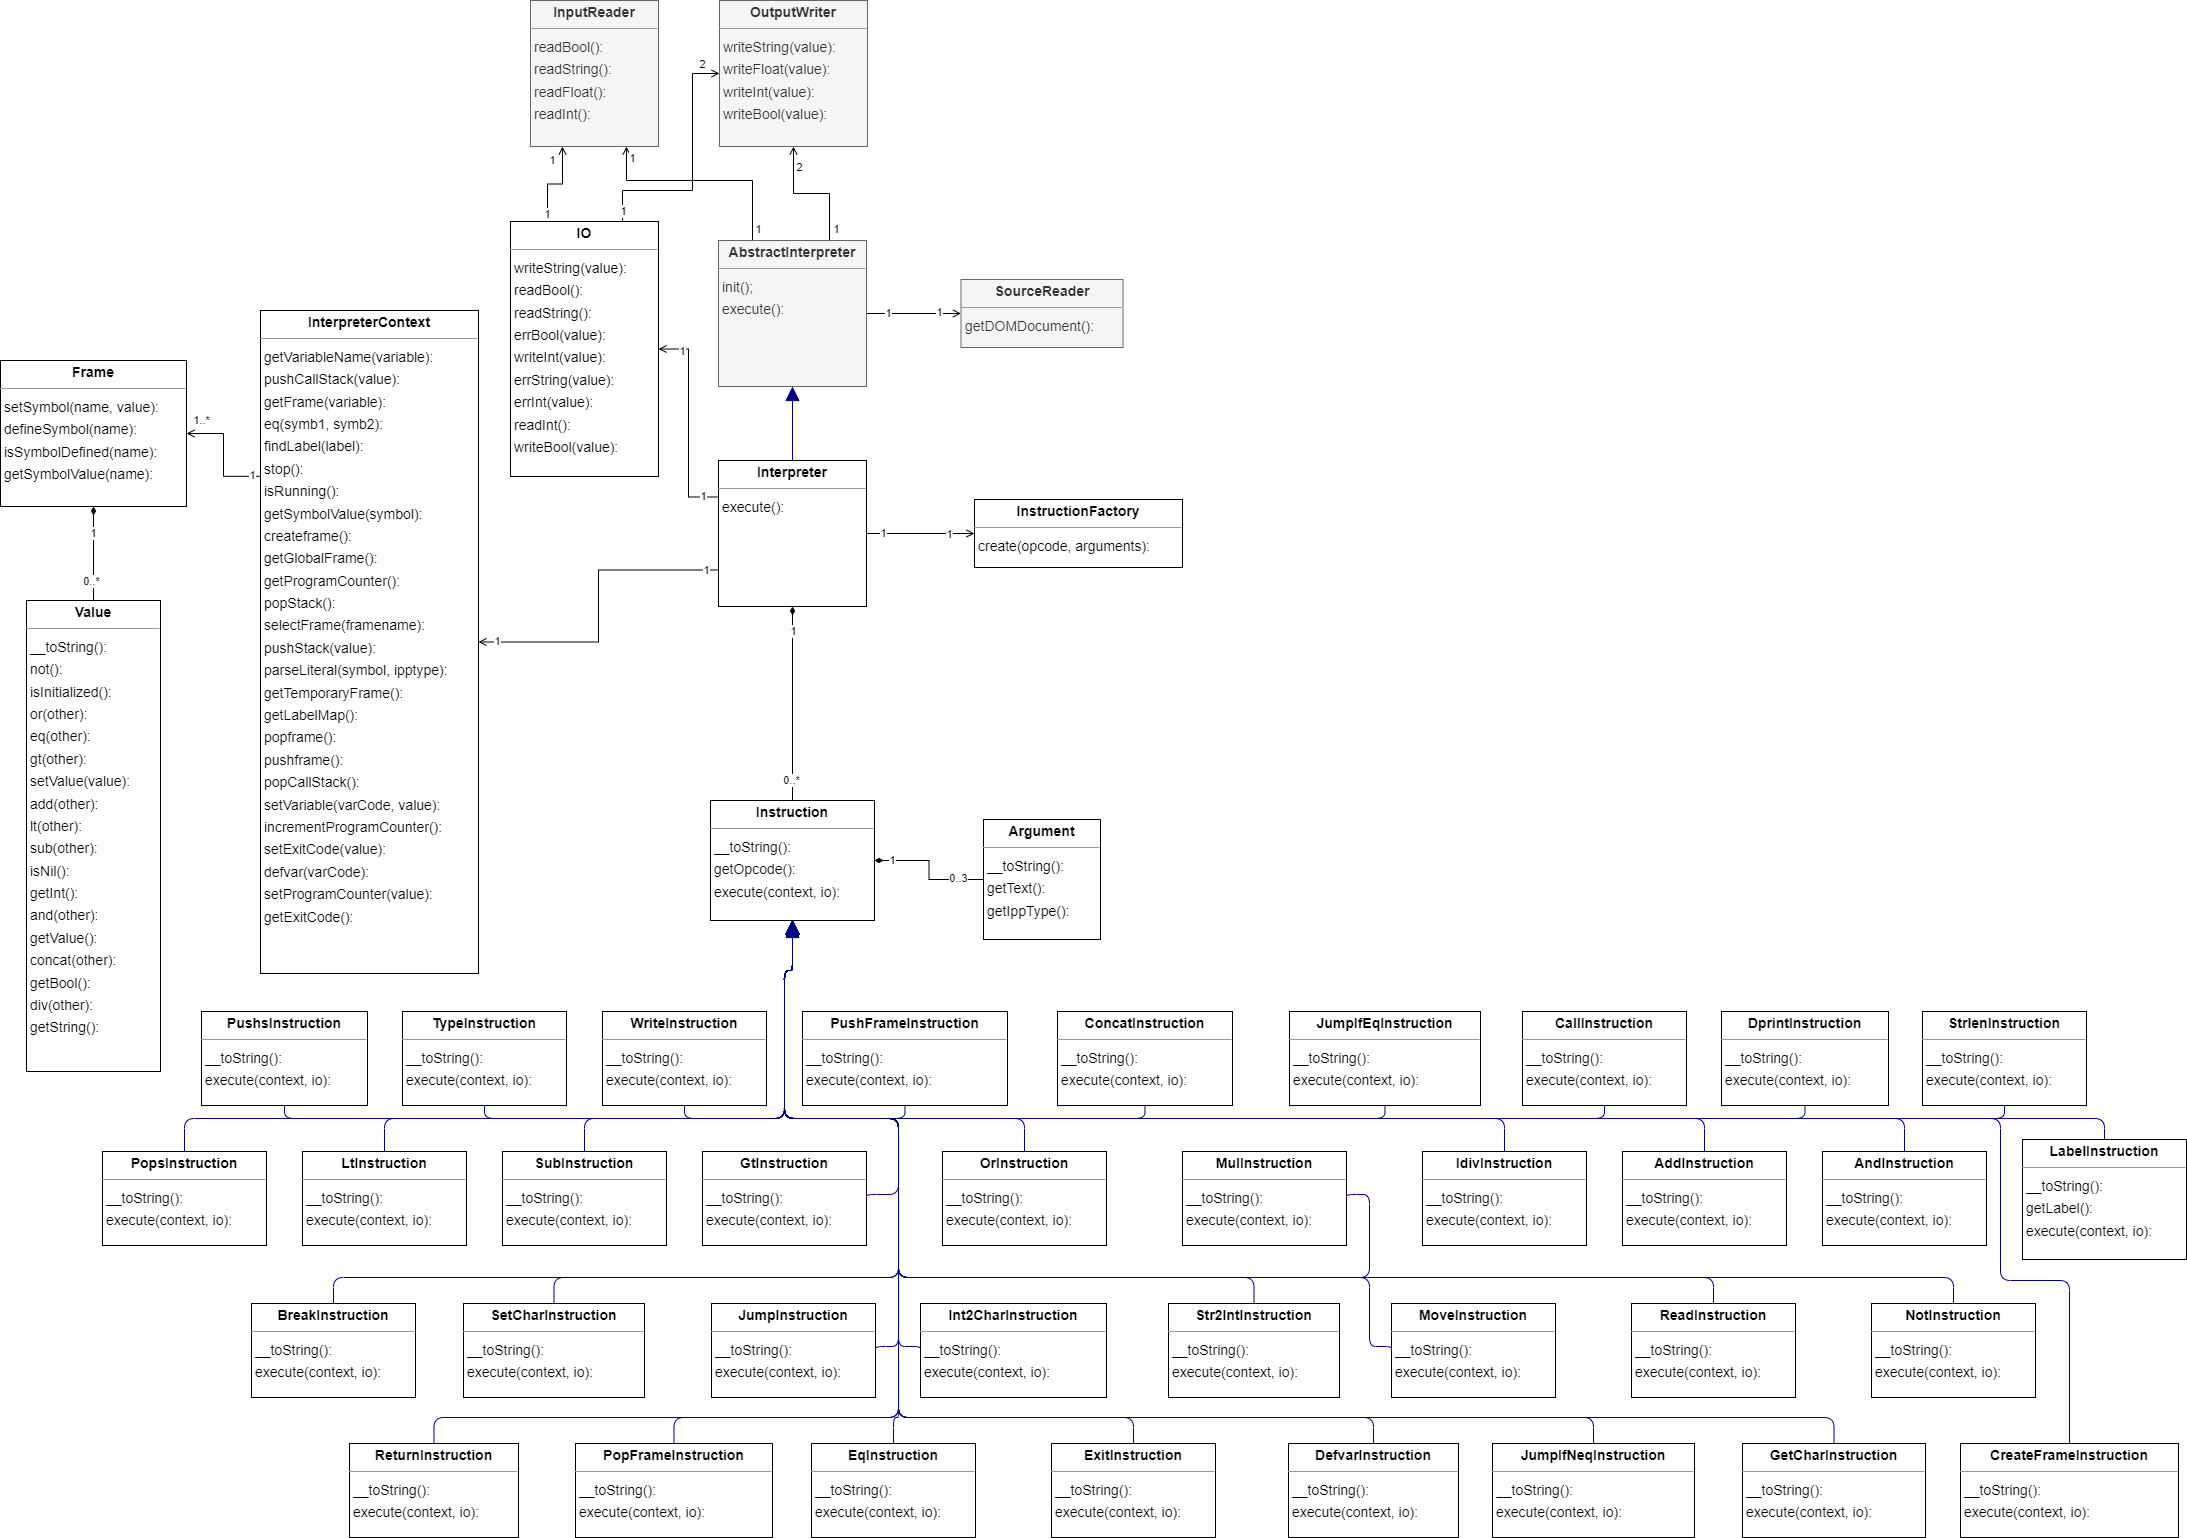
\includegraphics[width=\textwidth]{diagram.png}
  \caption{Diagram tříd.}
  \label{fig:diagram}
\end{figure}

\end{document}
